\documentclass[11pt,a4paper]{article}
\usepackage[margin=2.4cm]{geometry}
\usepackage[T1]{fontenc}
\usepackage{lmodern,booktabs,graphicx,float,listings,xcolor,caption,array}
\usepackage[colorlinks=true,linkcolor=blue!50!black,urlcolor=blue!50!black]{hyperref}
\sloppy
\lstset{basicstyle=\ttfamily\footnotesize,breaklines=true,frame=single,backgroundcolor=\color{black!3}}
\graphicspath{{figures/}}
\newcommand{\mlkem}{ML-KEM-768}

\title{Post-Quantum Hybrid TLS Gateway for IoT\\[2pt]
\large Design, implementation and measurement of a lightweight ML-KEM / X25519 TLS~1.3 proxy for MQTT and HTTP}
\author{Vishwas N.\\ M.Tech, Digital Electronics and Communication, MSRIT}
\date{\today}

\begin{document}
\maketitle

\begin{abstract}
Large quantum computers running Shor's algorithm would break RSA and elliptic-curve
cryptography, and adversaries can already record today's traffic to decrypt it later
(``harvest now, decrypt later''). NIST has standardised ML-KEM (FIPS~203) and ML-DSA
(FIPS~204), but their keys and ciphertexts are an order of magnitude larger than
classical ones, which worries designers of constrained IoT systems. This project builds
a small TLS~1.3 terminating gateway that fronts an unmodified Mosquitto MQTT broker and
an HTTP backend, and offers three key-exchange profiles: classical X25519, hybrid
X25519MLKEM768, and pure \mlkem. We verify on the wire that the post-quantum groups are
negotiated, and measure handshake latency, bytes, CPU and memory. In our loopback
measurements the post-quantum key exchange adds roughly 2.3~kB to the handshake (about
$2.9\times$ the classical total) while the computation cost stays within a small
fraction of a millisecond. The dominant IoT-relevant cost is therefore bandwidth and
packet size, not CPU.
\end{abstract}

\section{Problem and motivation}
IoT nodes are expected to live for 10--20 years, so devices deployed now will outlast the
arrival of cryptographically relevant quantum computers. Confidentiality of data in
transit is the urgent part: a recorded handshake protected only by ECDH can be broken
retroactively. Authentication (signatures) is less urgent because it only has to resist
forgery \emph{at the time of the handshake}. This asymmetry motivates the common
migration order: \textbf{key exchange first} (hybrid), signatures later.

\section{System design}
\begin{figure}[H]\centering
\begin{lstlisting}
 edge node --TLS1.3 (X25519MLKEM768)--> [ PQC gateway ] --plain--> Mosquitto :1883
 edge node --TLS1.3 (X25519MLKEM768)--> [ PQC gateway ] --plain--> HTTP API  :8000
                  untrusted network        trusted/private network
\end{lstlisting}
\caption{Gateway architecture. The broker and backend are unchanged and unreachable from outside.}
\end{figure}

\paragraph{Gateway.} \texttt{gateway/pqc\_gateway.py} is an asyncio TCP proxy that terminates
TLS~1.3 (minimum version pinned) and relays bytes to an upstream, so it secures MQTT, HTTP,
or any other TCP protocol. It exports JSON statistics (connections, bytes, RSS, CPU).
The key-exchange groups are \emph{not} in the code: they come from an OpenSSL configuration
file chosen at start-up (Table~\ref{tab:profiles}), so the same binary runs all three profiles.

\begin{table}[H]\centering\small
\begin{tabular}{lll}\toprule
Profile & OpenSSL \texttt{Groups} & Wire codepoint\\\midrule
classical & \texttt{X25519:secp256r1} & \texttt{0x001d}\\
hybrid & \texttt{X25519MLKEM768:X25519} & \texttt{0x11ec}\\
pqc & \texttt{MLKEM768} & \texttt{0x0201}\\\bottomrule
\end{tabular}
\caption{Gateway profiles. The hybrid profile keeps an X25519 fallback so legacy nodes can
still connect during migration; the pure profile refuses them by design.}\label{tab:profiles}
\end{table}

\paragraph{Why hybrid.} X25519MLKEM768 concatenates an X25519 share with an ML-KEM-768
share and derives the secret from both, so the session is safe if \emph{either} primitive
holds. This hedges against an undiscovered weakness in the young lattice scheme.

\paragraph{Edge nodes.} \texttt{edge/edge\_node.py} is a dependency-free simulated sensor that
publishes telemetry over MQTT~3.1.1 (own minimal client) or HTTPS. In Docker it runs under
CPU and memory limits (default 0.25 CPU, 64~MB) to emulate a constrained device.

\paragraph{Instrumentation.} \texttt{analysis/handshake\_probe.py} performs a handshake over
an in-memory TLS BIO, captures every byte, and parses the ClientHello/ServerHello. This
gives Wireshark-equivalent evidence without root privileges. \texttt{analysis/pcap\_clienthello.py}
applies the same parser to real \texttt{.pcap}/\texttt{.pcapng} files from tcpdump or Wireshark.

\section{Experimental setup}
\begin{itemize}
\item Stack: Python~3.13 with OpenSSL~3.5.9 (native ML-KEM, no external provider needed).
      The \texttt{cryptography} 50 library supplies ML-KEM/ML-DSA primitives; an optional
      \texttt{liboqs-python} backend is supported by the primitive benchmark.
\item Handshake benchmark: 150 measured handshakes per profile after 5 warm-up, each a full
      (non-resumed) TLS~1.3 handshake with an ECDSA P-256 server certificate.
\item Measurements reported here were taken on \textbf{loopback, with no CPU limit, in a cloud
      sandbox}. They quantify computation and byte overhead, but contain \emph{no network
      latency or packet loss}. Constrained-device results require running
      \texttt{make bench-docker} (CPU-limited containers) or the same scripts on a Raspberry~Pi.
\end{itemize}

\section{Results}
\subsection{Wire-level verification}
Probing the three gateways confirmed that each negotiates the intended group:

\begin{table}[H]\centering\footnotesize
\resizebox{\textwidth}{!}{\begin{tabular}{lllrr}\toprule
Profile & Client offers & Server selects & key\_share (client) & ClientHello\\\midrule
classical & x25519, secp256r1 & x25519 & 32 B & 232 B\\
hybrid & X25519MLKEM768, x25519 & X25519MLKEM768 & 1216 B & 1416 B\\
pqc & MLKEM768 & MLKEM768 & 1184 B & 1374 B\\\bottomrule
\end{tabular}}
\caption{Observed negotiation. $1216 = 32 + 1184$ (X25519 + \mlkem{} encapsulation key).
The server's hybrid share is 1120~B ($32 + 1088$-byte ciphertext).}
\end{table}
A classical-only client connecting to the pure-PQC gateway fails the handshake, as intended.
Note that the ClientHello grows from 232~B to 1416~B and therefore no longer fits in a
single small packet on links with a reduced MTU (see Discussion).

\subsection{Handshake cost}
\begin{table}[H]\centering\footnotesize
\resizebox{\textwidth}{!}{\begin{tabular}{lrrrrrrr}
\toprule
Profile & Median (ms) & p95 (ms) & ClientHello (B) & Total (B) & Client CPU (ms) & GW CPU (ms) & GW RSS (MB)\\
\midrule
classical & 1.32 & 1.81 & 232 & 1201 & 1.49 & 1.16 & 26.0\\
hybrid & 1.54 & 1.81 & 1416 & 3473 & 1.58 & 1.35 & 26.4\\
pqc & 1.34 & 1.58 & 1374 & 3400 & 1.18 & 1.23 & 26.2\\
\bottomrule
\end{tabular}
}
\caption{Handshake benchmark summary (loopback, 150 handshakes per profile).}\label{tab:hs}
\end{table}
\begin{figure}[H]\centering
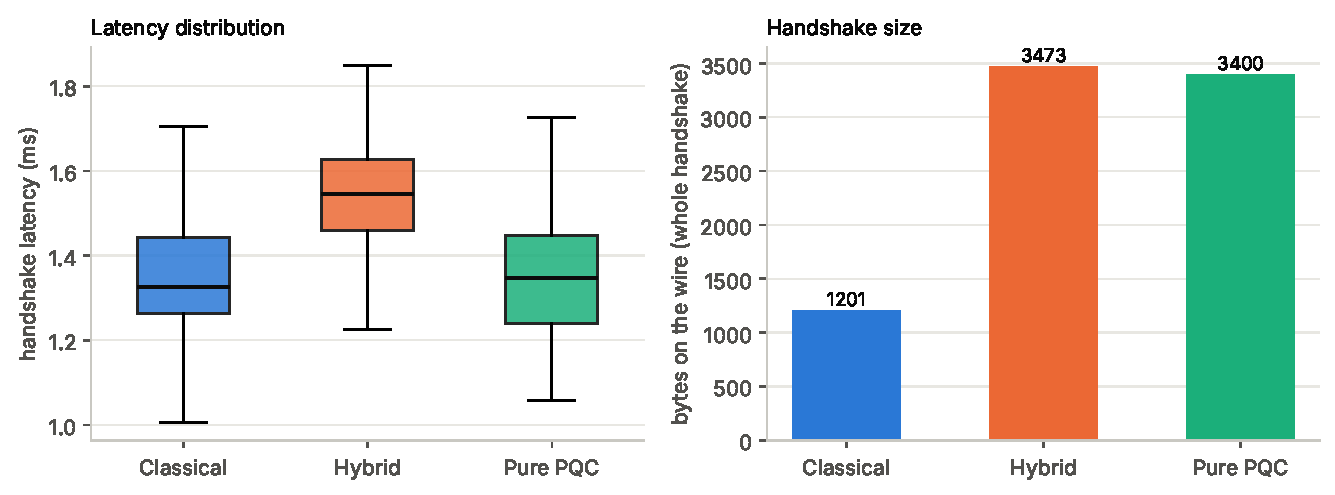
\includegraphics[width=\textwidth]{fig_handshake}
\caption{Latency distribution (box: quartiles, line: median, whiskers: range without outliers)
and total handshake bytes.}
\end{figure}
Total handshake bytes rise from 1201~B to 3473~B (hybrid) and 3400~B (pure PQC). Median latency
differences between the profiles (1.3--1.5~ms) are of the order of the run-to-run spread
and should not be over-interpreted: on loopback a single ML-KEM operation costs tens of
microseconds, far below the scheduling noise of a Python client. The bytes are the
robust signal.

\begin{figure}[H]\centering
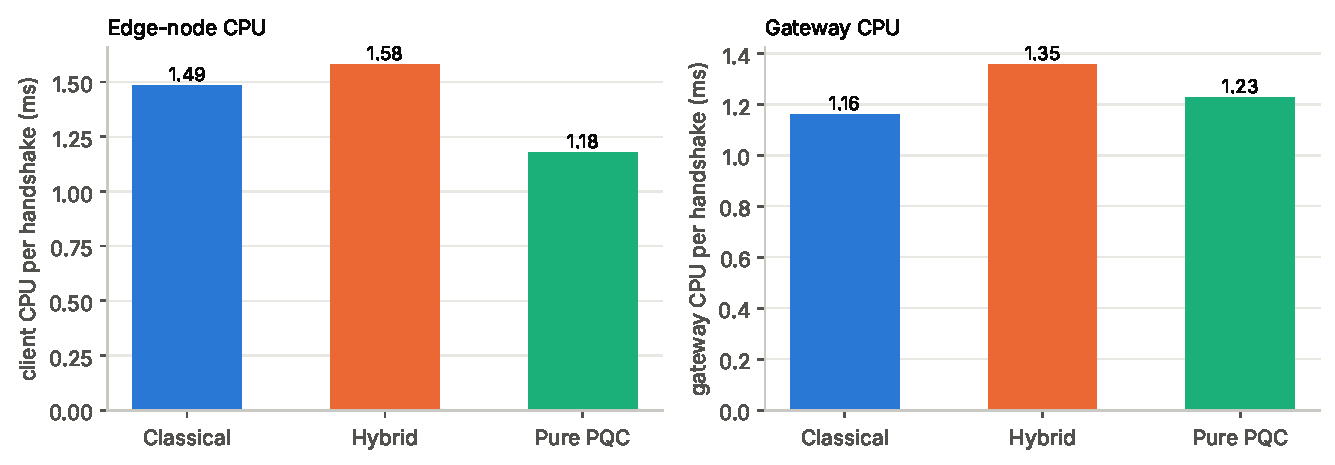
\includegraphics[width=\textwidth]{fig_cpu}
\caption{CPU time per handshake on the client and on the gateway process.}
\end{figure}
Gateway resident memory is about 26~MB in all profiles; the PQC groups do not measurably
change the steady-state footprint of the proxy.

\subsection{Primitive cost and sizes}
\begin{figure}[H]\centering
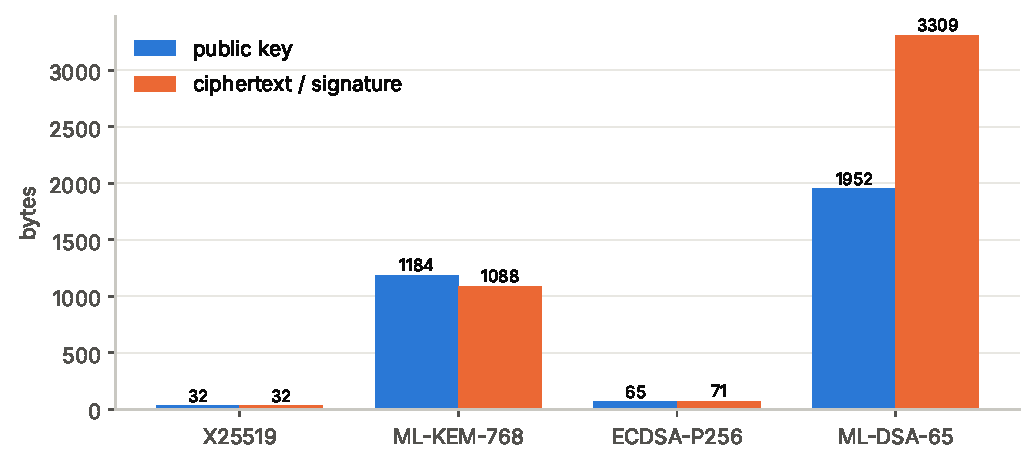
\includegraphics[width=0.78\textwidth]{fig_sizes}
\caption{Public key and ciphertext/signature sizes.}
\end{figure}
\begin{figure}[H]\centering
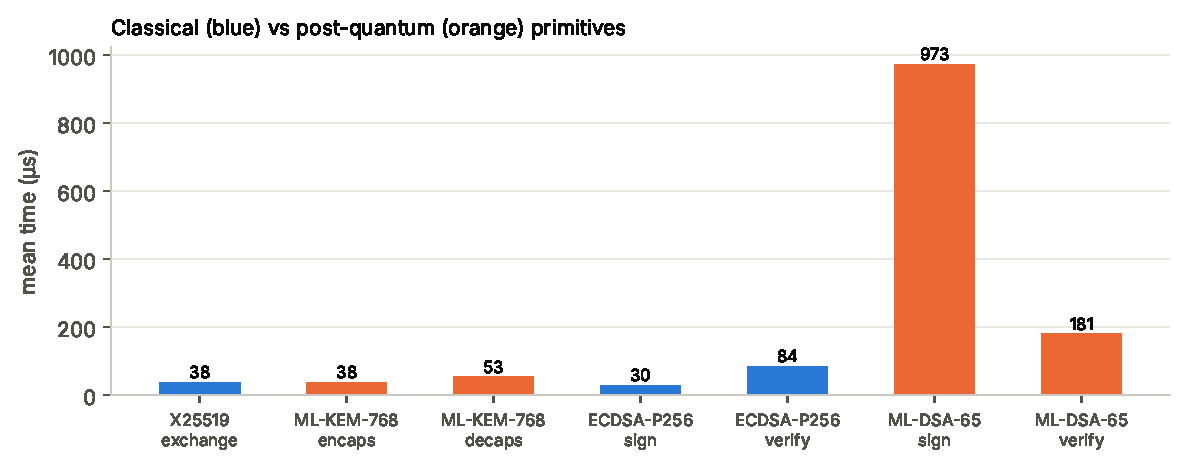
\includegraphics[width=0.9\textwidth]{fig_ops}
\caption{Mean time per operation. ML-KEM is competitive with X25519; ML-DSA signing is slower
than ECDSA P-256 signing but verification is of the same order.}
\end{figure}
ML-KEM-768 encapsulation and decapsulation (about 38 and 53~\textmu s here) are comparable
to an X25519 operation (about 38~\textmu s). ML-DSA-65 produces 3309-byte signatures and
1952-byte public keys, versus 71 and 65 bytes for ECDSA P-256; a full ML-DSA certificate chain
would add many kilobytes to the handshake.

\section{Discussion}
\paragraph{Bandwidth, not CPU, is the constraint.} On a modern core the arithmetic is cheap.
For a battery-powered radio the extra ${\approx}2.3$~kB per full handshake costs energy
and, on LoRaWAN/NB-IoT/802.15.4 class links with small MTUs, causes fragmentation or is
infeasible. The mitigations are standard: keep connections open (MQTT is long-lived),
use TLS session resumption so the large key share is not resent, and terminate TLS at a
nearby gateway.

\paragraph{Gateway pattern.} Concentrating PQC at the gateway lets legacy broker and
backend software stay unmodified, and the hybrid profile allows a gradual fleet migration.
The gateway is a high-value target and a single point of failure; it should run with a
hardened configuration and, in production, mutual TLS (supported via \texttt{--client-ca}).

\paragraph{Signatures.} The measured handshakes authenticate with ECDSA. This protects
confidentiality against harvest-now-decrypt-later, but a future quantum adversary could forge
an ECDSA-authenticated server \emph{at that time}. ML-DSA certificates are supported by
\texttt{certs/gen\_certs.sh} when the local OpenSSL can generate them, but handshake
benchmarks with ML-DSA chains were \textbf{not} part of these measurements.

\section{Limitations}
\begin{itemize}
\item Loopback and unconstrained CPU: no network effects, and a desktop-class CPU.
\item Python client/gateway: absolute latencies are dominated by interpreter and syscall
      overhead; they are not representative of a C firmware stack.
\item Only the key exchange was varied end-to-end; the ML-DSA data are primitive-level.
\item Docker and Raspberry~Pi runs are provided as scripts but are not part of the numbers above.
\item Energy was not measured.
\end{itemize}

\section{Reproducing the work}
\begin{lstlisting}
make certs              # demo CA + server certificate
make up                 # mosquitto, backend, 3 gateways (docker compose)
make bench-docker       # CPU-limited edge container -> results/*.csv
make figures            # regenerate figures and tables
make capture PROFILE=hybrid PORT=8884   # tcpdump + automatic verification
make report             # build this PDF
\end{lstlisting}
Wireshark filters for the screenshots are in \texttt{capture/WIRESHARK.md}.

\section{Conclusion}
A TLS~1.3 gateway using hybrid X25519MLKEM768 secures MQTT and HTTP IoT traffic against
harvest-now-decrypt-later attacks with modest computation overhead. The price is about
2.3~kB of extra handshake data, which matters for low-bandwidth links but not for the CPU.
Next steps: measurements on real constrained hardware, session-resumption savings, and an
ML-DSA/composite-certificate handshake.

\begin{thebibliography}{9}
\bibitem{fips203} NIST, FIPS 203: Module-Lattice-Based Key-Encapsulation Mechanism Standard, 2024.
\bibitem{fips204} NIST, FIPS 204: Module-Lattice-Based Digital Signature Standard, 2024.
\bibitem{rfc8446} E.~Rescorla, RFC 8446: The Transport Layer Security (TLS) Protocol Version 1.3, 2018.
\bibitem{hybrid} IETF TLS WG, Post-quantum hybrid ECDHE-MLKEM key agreement for TLSv1.3 (draft-ietf-tls-ecdhe-mlkem).
\bibitem{oqs} Open Quantum Safe project, liboqs and oqs-provider, \url{https://openquantumsafe.org}.
\end{thebibliography}
\end{document}
